% Dải tiêu đề mục Bài tập 2.5 với 4 vạch cyan hai bên đặc trưng
\noindent
\raisebox{2pt}{%
  \parbox[c]{26pt}{%
    \color{stewartcyan}%
    \hrule height 0.6pt\vspace{2.2pt}%
    \hrule height 0.6pt\vspace{2.2pt}%
    \hrule height 0.6pt\vspace{2.2pt}%
    \hrule height 0.6pt%
  }%
}%
\hspace{8pt}%
\parbox[c]{120pt}{%
  \fontsize{19}{21}\selectfont\bfseries%
  \textcolor{stewartcyan}{2.5}\hspace{6pt}%
  {\color{stewartcyan}\vrule width 1.2pt height 16pt depth 2pt}\hspace{6pt}%
  \textsf{Bài tập}%
}%
\hspace{4pt}%
\raisebox{2pt}{%
  \parbox[c]{\dimexpr\linewidth-26pt-8pt-120pt-4pt\relax}{%
    \color{stewartcyan}%
    \hrule height 0.6pt\vspace{2.2pt}%
    \hrule height 0.6pt\vspace{2.2pt}%
    \hrule height 0.6pt\vspace{2.2pt}%
    \hrule height 0.6pt%
  }%
}
\vspace{8pt}

% Bố cục 2 cột bài tập cân xứng tuyệt đối
\noindent
\begin{minipage}[t]{0.485\textwidth}
\begin{enumerate}[label=\textbf{\arabic*.}, leftmargin=15pt, itemsep=5pt, topsep=0pt]
\item Viết một phương trình thể hiện sự kiện rằng hàm số $f$ liên tục tại số $4$.

\item Nếu $f$ liên tục trên $(-\infty, \infty)$, ta có thể nói gì về đồ thị của nó?

\item 
\begin{enumerate}[label=\textnormal{(\alph*)}, leftmargin=15pt, itemsep=2pt, topsep=1pt]
  \item Từ đồ thị đã cho của $f$, hãy chỉ ra các số mà tại đó $f$ gián đoạn và giải thích tại sao.
  \item Với mỗi số đã chỉ ra ở phần (a), hãy xác định xem $f$ liên tục bên phải, bên trái, hay không liên tục về phía nào.
\end{enumerate}
\vspace{2pt}
\begin{center}
  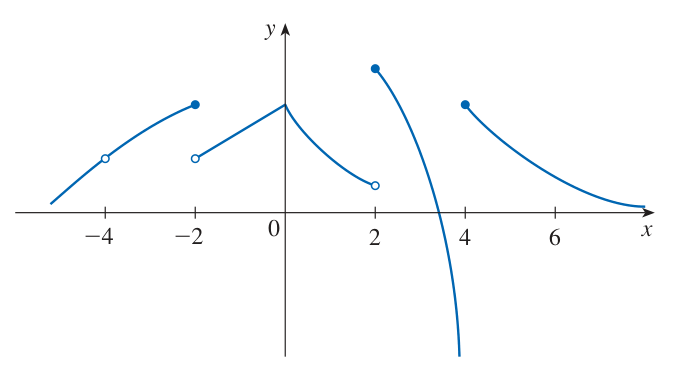
\includegraphics[width=0.96\linewidth]{images/p0159_fig1.png}
\end{center}
\vspace{-2pt}

\item Từ đồ thị đã cho của $g$, hãy chỉ ra các số mà tại đó $g$ gián đoạn và giải thích tại sao.
\vspace{2pt}
\begin{center}
  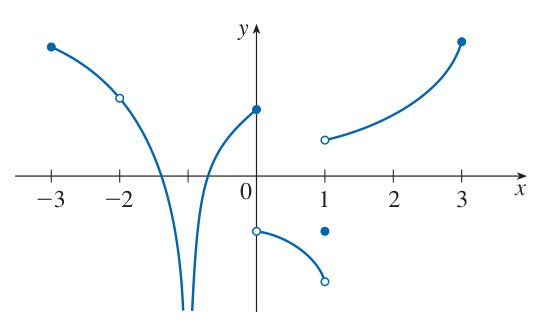
\includegraphics[width=0.88\linewidth]{images/p0159_fig2.png}
\end{center}
\vspace{-2pt}
\end{enumerate}

\noindent
\textbf{\textsf{\color{stewartcyan}5--6}}\enskip Cho đồ thị của một hàm số $f$.
\begin{enumerate}[label=\textnormal{(\alph*)}, leftmargin=15pt, itemsep=1.5pt, topsep=2pt]
  \item Tại những số $a$ nào thì $\lim\limits_{x \to a} f(x)$ không tồn tại?
  \item Tại những số $a$ nào thì $f$ không liên tục?
  \item Tại những số $a$ nào thì $\lim\limits_{x \to a} f(x)$ tồn tại nhưng $f$ không liên tục tại $a$?
\end{enumerate}
\vspace{1pt}
\begin{center}
  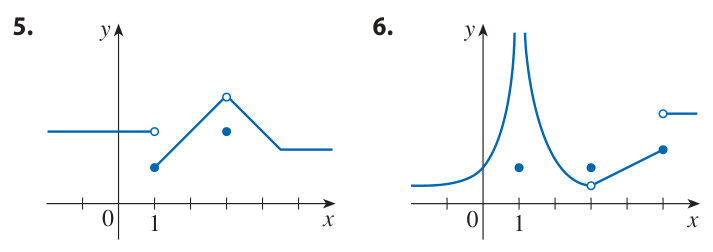
\includegraphics[width=\linewidth]{images/p0159_fig3.png}
\end{center}
\vspace{2pt}

\noindent{\color{stewartcyan}\rule{\linewidth}{0.5pt}}
\vspace{4pt}

\noindent
\textbf{\textsf{\color{stewartcyan}7--10}}\enskip Phác thảo đồ thị của một hàm số $f$ xác định trên $\mathbb{R}$ và liên tục ở mọi nơi ngoại trừ các điểm gián đoạn đã nêu.
\vspace{3pt}

\begin{enumerate}[label=\textbf{\arabic*.}, leftmargin=15pt, itemsep=4pt, topsep=0pt, start=7]
\item Điểm gián đoạn khử được tại $-2$, điểm gián đoạn vô hạn tại $2$
\item Điểm gián đoạn bước nhảy tại $-3$, điểm gián đoạn khử được tại $4$
\end{enumerate}
\end{minipage}%
\hfill
\begin{minipage}[t]{0.485\textwidth}
\begin{enumerate}[label=\textbf{\arabic*.}, leftmargin=15pt, itemsep=4pt, topsep=0pt, start=9]
\item Gián đoạn tại $0$ và $3$, nhưng liên tục bên phải tại $0$ và liên tục bên trái tại $3$

\item Chỉ liên tục bên trái tại $-1$, không liên tục cả bên trái lẫn bên phải tại $3$
\end{enumerate}

\vspace{4pt}
\noindent{\color{stewartcyan}\rule{\linewidth}{0.5pt}}
\vspace{4pt}

\begin{enumerate}[label=\textbf{\arabic*.}, leftmargin=15pt, itemsep=5pt, topsep=0pt, start=11]
\item Mức phí $T$ phải trả khi lái xe trên một đoạn đường thu phí nhất định là \$5, ngoại trừ vào các giờ cao điểm (từ 7 giờ sáng đến 10 giờ sáng và từ 4 giờ chiều đến 7 giờ tối) khi mức phí là \$7.
\begin{enumerate}[label=\textnormal{(\alph*)}, leftmargin=15pt, itemsep=2pt, topsep=2pt]
  \item Phác thảo đồ thị của $T$ theo biến thời gian $t$, được tính bằng số giờ kể từ nửa đêm.
  \item Thảo luận về các điểm gián đoạn của hàm số này và ý nghĩa của chúng đối với một người tham gia giao thông trên tuyến đường đó.
\end{enumerate}

\item Giải thích tại sao mỗi hàm số sau liên tục hoặc gián đoạn.
\begin{enumerate}[label=\textnormal{(\alph*)}, leftmargin=15pt, itemsep=2pt, topsep=2pt]
  \item Nhiệt độ tại một địa điểm cụ thể theo hàm của thời gian
  \item Nhiệt độ tại một thời điểm cụ thể theo hàm của khoảng cách về phía tây tính từ Thành phố New York
  \item Độ cao so với mực nước biển theo hàm của khoảng cách về phía tây tính từ Thành phố New York
  \item Chi phí của một chuyến đi taxi theo hàm của quãng đường di chuyển
  \item Cường độ dòng điện trong mạch thắp sáng của một căn phòng theo hàm của thời gian
\end{enumerate}
\end{enumerate}

\vspace{3pt}
\noindent{\color{stewartcyan}\rule{\linewidth}{0.5pt}}
\vspace{3pt}

\noindent
\textbf{\textsf{\color{stewartcyan}13--16}}\enskip Dùng định nghĩa tính liên tục và các tính chất của giới hạn để chứng minh rằng hàm số liên tục tại số $a$ đã cho.
\vspace{3pt}

\begin{enumerate}[label=\textbf{\arabic*.}, leftmargin=15pt, itemsep=5pt, topsep=0pt, start=13]
\item $f(x) = 3x^2 + (x + 2)^5, \qquad a = -1$
\item $g(t) = \dfrac{t^2 + 5t}{2t + 1}, \qquad a = 2$
\item $p(v) = 2\sqrt{3v^2 + 1}, \qquad a = 1$
\item $f(r) = \sqrt[3]{4r^2 - 2r + 7}, \qquad a = -2$
\end{enumerate}

\vspace{3pt}
\noindent{\color{stewartcyan}\rule{\linewidth}{0.5pt}}
\vspace{3pt}

\noindent
\textbf{\textsf{\color{stewartcyan}17--18}}\enskip Dùng định nghĩa tính liên tục và các tính chất của giới hạn để chứng minh rằng hàm số liên tục trên khoảng đã cho.
\vspace{3pt}

\begin{enumerate}[label=\textbf{\arabic*.}, leftmargin=15pt, itemsep=5pt, topsep=0pt, start=17]
\item $f(x) = x + \sqrt{x - 4}, \qquad [4, \infty)$
\item $g(x) = \dfrac{x - 1}{3x + 6}, \qquad (-\infty, -2)$
\end{enumerate}

\vspace{3pt}
\noindent{\color{stewartcyan}\rule{\linewidth}{0.5pt}}
\vspace{3pt}

\noindent
\textbf{\textsf{\color{stewartcyan}19--24}}\enskip Giải thích tại sao hàm số gián đoạn tại số $a$ đã cho. Phác thảo đồ thị của hàm số.
\vspace{3pt}

\begin{enumerate}[label=\textbf{\arabic*.}, leftmargin=15pt, itemsep=6pt, topsep=0pt, start=19]
\item $f(x) = \dfrac{1}{x + 2}, \qquad a = -2$
\item $f(x) = \begin{cases} \dfrac{1}{x + 2} & \text{nếu } x \ne -2 \\[6pt] 1 & \text{nếu } x = -2 \end{cases} \qquad a = -2$
\end{enumerate}
\end{minipage}
